\documentclass{beamer}

\usepackage{minted}
\usepackage{tikz}

\newcommand*\circled[1]{\tikz[baseline=(char.base)]{\node[shape=circle,fill,inner sep=2pt] (char) {\textcolor{white}{#1}};}} % chktex 36


\usepackage[orientation=portrait,size=a1,scale=1.0]{beamerposter}
\usetheme{JuelichPoster}

\setbeamertemplate{partner1}{
\includegraphics{img/cscs}}
% TODO Add HBP and/or eBrains here

\begin{document}
\begin{frame}[t, fragile]
  \frametitle{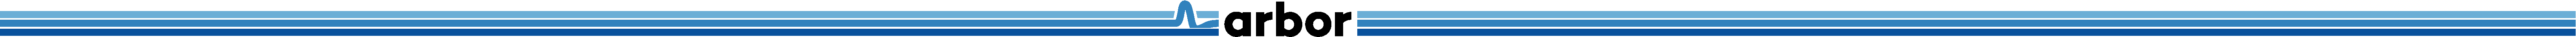
\includegraphics[width=\linewidth]{img/arbor-lines-proto-colour-full}}
  \framesubtitle{A morphologically detailed neural network simulation library for modern high performance computer architectures.\\
    \tiny{Nora Abi Akar, Ben Cumming, Stuart Yates (CSCS); Thorsten Hater, Brent Huisman, Anne Küsters (Forschungszentrum Jülich)}}

  \begin{columns}
    \begin{column}{0.65\textwidth}
      We present recent developments in Arbor, a library for the simulation of
      morphologically detailled neurons and networks thereof. Arbor places strong
      emphasis on performance, portability, and usability. It can exploit modern
      architectures based on super-scalar multi-core processors and GPU accelerators.
      We will showcase some of the features added to Arbor since the last release and
      how they can used to almost directly import single cell models from the Allen
      Brain Atlas database.
    \end{column}
    \begin{column}{0.3\textwidth}
      \begin{block}{Where to find us}
        \begin{description}
          \item[Contact] arbor-sim@fz-juelich.de
          \item[Source code] github.com/arbor-sim/arbor
          \item[Documentation] arbor.readthedocs.io
        \end{description}
      \end{block}
    \end{column}
  \end{columns}

  \textbf{{\large\structure{New Features}}}\\
  \begin{columns}[onlytextwidth]
    \begin{column}{.49\linewidth}
      \textbf{\structure{Morphology}}\\
    \end{column}
    \begin{column}{.49\linewidth}
      \textbf{\structure{Mechanism Catalogues}}\\
      We provide an interface to collections of \emph{mechanisms} which describe
      processes both associated with an area density like ion channels and
      localised like synapses. These mechanisms are described in the NMODL DSL
      and translated into plain or vectorised C++ and CUDA for execution on GPUs.

      In particular we currently offer two catalogues, one, called
      \emph{default} comprising basic functionality, e.g.\ a passive leak and
      secondly the \emph{allen} catalogue which is a collection of mechanisms
      obtained from the Brain Atlas\cite{Allen Mouse Brain Atlas}.
      These have been heavily optimised, as they form the basis for the V1
      network model \cite{Allen V1}.

      Catalogues are built at compile time and can be accessed in the simulation
      to provide the mechanisms used in the respective model. Further, they can
      be composed into compound catalogues, where name clashes are avoided via
      an optional prefix.

      \textbf{\structure{Spherical Somata}}\\
    \end{column}
  \end{columns}
  \textbf{{\large\structure{Running an Allen Brain Atlas Model}}}\\
  \begin{columns}[onlytextwidth]
    \begin{column}{.49\linewidth}
      The code snippet on the right is complete except the parsing and plotting
      steps; it is available in full together with this poster
      at~\cite{my-source}. While the electro-physiological data is supplied as a
      JSON file in all instances, the structure as some variation. Thus, the
      parsing cannot be standardised. We comment on some of the important steps
      \begin{itemize}
        \item[\circled{1}] load SWC structure from the download
        \item[\circled{2}] assign labels to geometry
        \item[\circled{3}] build a cell description from labels and geometry
        \item[\circled{4}] parse the electro-physiological properties supplied in the download and assign to regions
        \begin{itemize}
          \item set physical properties: $T$, $V_{m}$, $R_{a}$, $C_{m}$
          \item define ion dynamics reversal potentials
        \end{itemize}
        \item[\circled{5}] Attach to the soma's center
        \begin{itemize}
          \item current clamp; rectangular stimulus of $150\,pA$ from $200\,ms$ to $1200\,ms$
          \item voltage probe; sampling with $200\,kHz$
          \item spike detector; triggering at $V=-40\,mV$
        \end{itemize}
        \item[\circled{6}] convert the cell description into a runnable simulation
        \item[\circled{7}] set mechanism catalogue comprising the defaults and Allen DB mechanisms.
        \item[\circled{8}] run the simulation for $1400\,ms$ with time step $\Delta t = 0.005\,ms$
      \end{itemize}
      \begin{figure}[H]
        \centering
        \includegraphics{src/arbor.pdf}
      \end{figure}
      The reference solution was obtained using the allensdk Python package with
      the default Neuron backend~\cite{allensdk, neuron}. A minor modification
      was made to suppress editing of the axon at load time of the geometric
      information. For comparable simulations, we instead performed this
      manipulation by hand once and stored the result in the SWC input. We
      observe a minor deviation from the reference run, which is explained by
      different discretisations.

      The elapsed wall clock times for only the simulation steps are $14.7\,s$
      with the code on the right and $121.8\,s$ for the reference solution;
      yielding a speed-up of $8.25\times$ when using Arbor.
    \end{column}
    \begin{column}{.49\linewidth}
      \inputminted[escapeinside=!!]{python}{src/model.py}
    \end{column}
  \end{columns}
  \vspace*{5ex}
  \begin{columns}[onlytextwidth]
    \begin{column}{.49\linewidth}
      \textbf{\structure{Outlook}}\\
      \begin{itemize}
        \item Running V1 network model: This is the groundwork.
        \item SONATA
      \end{itemize}
    \end{column}
    \begin{column}{.49\linewidth}
      \textbf{\structure{Acknowledgements}}\\
      This research has received funding from the European Union's Horizon 2020
      Framework Programme for Research and Innovation under the Specific Grant
      Agreement No. 720270 (HBP SGA1), Specific Grant Agreement No. 785907 (HBP
      SGA2), and Specific Grant Agreement No. 945539 (HBP SGA3).
      
      \textbf{\structure{References}}\\
    \end{column}
  \end{columns}
\end{frame}
\end{document}
